%# -*- coding:utf-8 -*-
\documentclass[10pt,aspectratio=169,mathserif]{beamer}		
%设置为 Beamer 文档类型,设置字体为 10pt,长宽比为16:9,数学字体为 serif 风格

%%%%-----导入宏包-----%%%%
\usepackage{zju}			%导入 zju 模板宏包
\usepackage{ctex}			%导入 ctex 宏包,添加中文支持
\usepackage{amsmath,amsfonts,amssymb,bm,amsthm}   %导入数学公式所需宏包
\usepackage{color}			 %字体颜色支持
\usepackage{graphicx,hyperref,url}
\usepackage{metalogo}	% 非必须
\usepackage{ragged2e}
\usepackage{wrapfig}
\usepackage{caption}
\usepackage{tabularx}
\usepackage{booktabs}
\usepackage{calc}


\usepackage[
    style=gb7714-2015,
    gbcitelocal=chinese,   % Uncomment if you want \citeauthor{} in "et al." format. GitHub PR (#324)
    % gbpub=false,         % Uncomment if you do NOT want '[S.l. : s.n.]' in reference entries, GitHub Issue (#47)
    % gbnamefmt=lowercase, % Uncomment if you do NOT want uppercase author names in reference entries, GitHub Issue (#23)
]{biblatex}
\addbibresource{ref.bib}
%% 上文引用的包可按实际情况自行增删
%%%%%%%%%%%%%%%%%%
\usepackage{fontspec}
\usepackage{xeCJK}


% \setCJKmainfont{Source Han Sans SC}
\setbeamertemplate{caption}[numbered] % 图片添加编号


\beamertemplateballitem		%设置 Beamer 主题

%%%%------------------------%%%%%
\catcode`\。=\active         %或者=13
\newcommand{。}{.}				
%将正文中的“。”号转换为“.”。中文标点国家规范建议科技文献中的句号用圆点替代
%%%%%%%%%%%%%%%%%%%%%

%%%%----首页信息设置----%%%%
\title[局部间断伽辽金法的算法设计与应用]{局部间断伽辽金法的算法设计与应用}	
%%%%----标题设置


\author[鲁硕]{
  鲁硕 \\ 
  {\small \url{lushuo@zju.edu.cn}} \\ \medskip
  {指导老师:仲杏慧}
}
%%%%----个人信息设置

\institute[IOPP]{
  信息与计算科学 \\ 
  浙江大学}
%%%%----机构信息

\date[\today]{
  \today}
%%%%----日期信息
%%%%%%%%%%%%%%%%%%%%%%%%%%%%%%%%%%%%%%%%%%%%%%%%%%%%%%%%%%%%%%%%%%%%%
%%%% 文档开始
%%%%%%%%%%%%%%%%%%%%%%%%%%%%%%%%%%%%%%%%%%%%%%%%%%%%%%%%%%%%%%%%%%%%%
\begin{document}
\newlength{\llen}
\newlength{\slen}
\setlength{\llen}{\widthof{1.86}}
\setlength{\slen}{\widthof{1.86}}

\begin{frame}
	\titlepage
\end{frame}				%生成标题页


\begin{frame}
	%%  	\frametitle{提纲}
	\tableofcontents
\end{frame}				%生成提纲页

\section{研究背景与意义}
\begin{frame}
	\frametitle{研究背景与意义}
	\begin{itemize}
		\item 对于LDG法解决一维漂移-扩散(DD)模型和高场(HF)模型问题已经有了理论上的误差估计,但其正确性还缺少完善的验证。
		\item 我们的主要工作是验证补充多维度数值算例对比以及验证误差估计的正确性。
	\end{itemize}
\end{frame}
\section{预备知识}
\begin{frame}
	\frametitle{基础符号}
	\begin{itemize}
		\item 计算域I(本文取$[0, 0.6]$)的一个划分:$I_j = (x_{j-\frac{1}{2}},x_{j+\frac{1}{2}}),j=1,2,\cdots,N$。$\Delta x_j = x_{j+\frac{1}{2}}-x_{j-\frac{1}{2}},x_j = \frac{1}{2}(x_{j-\frac{1}{2}}+x_{j+\frac{1}{2}}), h = \max \limits_j \Delta x_j$。
		      \begin{equation*}
			      0 = x_{\frac{1}{2}} < x_{\frac{3}{2}} < \cdots < x_{N-\frac{1}{2}} < x_{N+\frac{1}{2}} = 0.6.
		      \end{equation*}
		\item 有限维计算空间$V_h^k = \{z:z|_{I_j} \in P^k(I_j)\}$,其中$P^k(I_j)$表示$I_j$上的k次多项式。
	\end{itemize}
\end{frame}

\section{DD模型}
\subsection{LDG离散DD模型}
\begin{frame}
	\frametitle{DD模型}
	漂移-扩散(DD)模型
	\begin{block}{DD模型}
		\begin{align}
			n_t - (\mu En)_x = \tau \theta n_{xx}, \label{eq:DD} \\
			\phi_{xx} = \frac{e}{\epsilon}(n - n_d),  \label{eq:poisson}
		\end{align}
		其中$x \in (0,1)$,第一个方程具有周期边界条件,势方程$\phi(0,t) = 0, \phi(1,t) = v_{bias}$具有Dirichlet边界条件。泊松方程\eqref{eq:poisson}是电势方程。

		在系统\eqref{eq:DD}-\eqref{eq:poisson},未知变量是电子浓度n和电势$\phi$,$E = -\phi_x$代表电场。其余物理量均已知。
	\end{block}
\end{frame}
\begin{frame}
	\frametitle{DD模型弱形式}
	引入辅助变量$q = \sqrt{\tau \theta }n_x$和测试函数$v,\omega, r, z \in V_h^k$,得到DD模型的弱形式:
	\begin{block}{弱形式}
		\begin{align}
			 & \int_{I_{j}} n_{t} v d x+\int_{I_{j}}(\mu E n+\sqrt{\tau \theta} q) v_{x} d x                                                                               \nonumber                                            \\
			 & \quad-(\mu E n+\sqrt{\tau \theta} q)_{j+\frac{1}{2}} v_{j+\frac{1}{2}}^{-}+(\mu E n+\sqrt{\tau \theta} q)_{j-\frac{1}{2}} v_{j-\frac{1}{2}}^{+}=0,            \label{eq:LDG:n}                                   \\
			 & \int_{I_{j}} q w d x+\int_{I_{j}} \sqrt{\tau \theta} n w_{x} d x-\sqrt{\tau \theta} n_{j+\frac{1}{2}} w_{j+\frac{1}{2}}^{-}+\sqrt{\tau \theta} n_{j-\frac{1}{2}} w_{j-\frac{1}{2}}^{+}=0, \label{eq:LDG:q}       \\
			 & -\int_{I_j}Er_x\rm{d}x + E_{j+\frac{1}{2}}r_{j+\frac{1}{2}}^- - E_{j-\frac{1}{2}}r_{j-\frac{1}{2}}^+ = -\frac{e}{\epsilon}\int_{I_j}(n-n_d)r\rm{d}x,                                       \label{DD:weakform:E} \\
			 & \int_{I_j} Ez \rm{d}x - \int_{I_j}\phi z_x \rm{d}x + \phi_{j+\frac{1}{2}}z_{j+\frac{1}{2}}^- - \phi_{j-\frac{1}{2}}z_{j-\frac{1}{2}}^+ = 0, \label{DD:weakform:phi}
		\end{align}
	\end{block}
\end{frame}
\begin{frame}
	\frametitle{DD模型LDG格式}
	将精确解$n, q, E$替换为数值解$n_h, q_h, E_h$,单元边界上的项替换为数值通量,得到:
	\begin{block}{DD模型半LDG格式}
		\begin{align}
			 & \int_{I_{j}}\left(n_h\right)_{t} v d x+\int_{I_{j}}\left(\mu E_h n_h+\sqrt{\tau \theta} q_h\right) v_{x} d x      \nonumber                                                                                                                    \\
			 & \quad-\left(\mu \widehat{E_h n_h}+\sqrt{\tau \theta} \hat{q}_{h}\right)_{j+\frac{1}{2}} v_{j+\frac{1}{2}}^{-}+\left(\mu \widehat{E_h n_h}+\sqrt{\tau \theta} \hat{q}_{h}\right)_{j-\frac{1}{2}} v_{j-\frac{1}{2}}^{+}=0, \label{eq:DDLDGn}     \\
			 & \int_{I_{j}} q_h w d x+\int_{I_{j}} \sqrt{\tau \theta} n_h w_{x} d x-\sqrt{\tau \theta} (\hat{n}_h)_{j+\frac{1}{2}} w_{j+\frac{1}{2}}^{-}+\sqrt{\tau \theta} (\hat{n}_h)_{j+\frac{1}{2}} w_{j-\frac{1}{2}}^{+}=0,            \label{eq:DDLDGq} \\
			 & E_h=\int_{0}^{x}-\frac{e}{\varepsilon}\left(n_h-n_{d}\right) d x+E_{0}-v_{\text {bias}},\label{eq:DDLDGE}
		\end{align}
	\end{block}
\end{frame}
\begin{frame}
	将精确解$n, q, E, \phi $替换为对应的数值解$n_h, q_h, E_h, \phi_h $,单元边界上的项替换为数值通量,得到:
	\begin{block}{DD模型LDG格式}
		\begin{align}
			 & \int_{I_{j}}\left(n_h\right)_{t} v d x+\int_{I_{j}}\left(\mu E_h n_h+\sqrt{\tau \theta} q_h\right) v_{x} d x      \nonumber                                                                                                                       \\
			 & \quad-\left(\mu \widehat{E_h n_h}+\sqrt{\tau \theta} \hat{q}_{h}\right)_{j+\frac{1}{2}} v_{j+\frac{1}{2}}^{-}+\left(\mu \widehat{E_h n_h}+\sqrt{\tau \theta} \hat{q}_{h}\right)_{j-\frac{1}{2}} v_{j-\frac{1}{2}}^{+}=0, \label{eq:IMEX:DD:n}     \\
			 & \int_{I_{j}} q_h w d x+\int_{I_{j}} \sqrt{\tau \theta} n_h w_{x} d x-\sqrt{\tau \theta} (\hat{n}_h)_{j+\frac{1}{2}} w_{j+\frac{1}{2}}^{-}+\sqrt{\tau \theta} (\hat{n}_h)_{j+\frac{1}{2}} w_{j-\frac{1}{2}}^{+}=0,            \label{eq:IMEX:DD:q} \\
			 & -\int_{I_j}E_hr_x\rm{d}x + (\hat{E}_h)_{j+\frac{1}{2}}r_{j+\frac{1}{2}}^- - (\hat{E}_h)_{j-\frac{1}{2}}r_{j-\frac{1}{2}}^+ = -\frac{e}{\epsilon}\int_{I_j}(n_h-n_d)r\rm{d}x,                                        \label{eq:IMEX:poisson:1}     \\
			 & \int_{I_j} E_hz \rm{d}x - \int_{I_j}\phi_h z_x \rm{d}x +  (\widehat{\phi}_h)_{j+\frac{1}{2}}z_{j+\frac{1}{2}}^- - (\widehat{\phi}_h)_{j-\frac{1}{2}}z_{j-\frac{1}{2}}^+ = 0.\label{eq:IMEX:poisson:2}
		\end{align}
	\end{block}
\end{frame}

%%%%%%%%%%%%%%%%%%%%%%%%%%
% 误差估计
%%%%%%%%%%%%%%%%%%%%%%%%%%
\subsection{误差估计}
\begin{frame}
	\frametitle{误差估计}
	我们定义:$||u||_{L^{\infty}(0,T;L^2)}  = \max \limits_{0 \leq t \leq T}||u^m||_{l^2(I)}$和$||u||_{L^2(0,T;L^2)} = (\int_{0}^{T}||u^m||_{L^2(I)}^2\Delta t)^{1/2}$。对于DD模型的三阶TVD LDG格式,我们有以下误差估计\cite{liu2010error}:
	\begin{theorem}[DD模型三阶TVD LDG格式误差估计]
		设$n, q$是光滑精确解,它们足够光滑且有有界导数。设$n_h, q_h$是半LDG格式\eqref{eq:DDLDGn}-\eqref{eq:DDLDGq}的数值解。相应的数值误差记为$e_{u}=u-u_{h}(u=n, q)$。如果有限元空间$V_{h}^{k}$是$k \geq 1$次分段多项式,则对于足够小的$h$,有以下误差估计成立:
		\begin{equation}
			\left\|n-n_h\right\|_{L^{\infty}\left(0, T ; L^{2}\right)}+\left\|q-q_h\right\|_{L^{2}\left(0, T ; L^{2}\right)} \leq C h^{k+\frac{1}{2}},
		\end{equation}
		其中常数$C$依赖于最终时间$T,k, \|n\|_{L^{\infty}\left(0, T ; H^{k+1}\right)}$和$\left\|n_{x}\right\|_{0, \infty}$。
	\end{theorem}
\end{frame}

\begin{frame}
	\frametitle{误差估计}
	对于一阶IMEX LDG格式,我们有以下误差估计\cite{liu2016analysis}:
	\begin{theorem}[一阶IMEX LDG格式误差估计]
		令$n^m,q^m$是在时间层级m的光滑精确解,它们足够光滑且有有界导数。令$n_h^m,q_h^m$是一阶IMEX LDG格式的数值解。如果有限元空间$V_h^k$是k$(k\geq  0)$阶间断多项式,那么对于足够小的h,存在与h无关的正常数C,使得下列误差估计成立
		\begin{equation}
			||n-n_h||_{L^{\infty}(0,T;L^2)} + ||q - q_h||_{L^2(0,T;L^2)} \leq C(h^{k+1} + \Delta t), \label{eq:IMEX:es:1}
		\end{equation}
		其中C依赖于最终时间$T,k,C_{\mu}$,反常数$C_2, ||n||_{L^{\infty}(0,T;H^{k+1})}, ||n_x||_{L^{\infty}}$和$||E||_{L^{\infty}}$。
	\end{theorem}
\end{frame}

\begin{frame}
	\frametitle{误差估计}
	对于二阶IMEX LDG格式,我们有以下误差估计\cite{liu2016analysis}:
	\begin{theorem}[二阶IMEX LDG格式误差估计]
		令$n^m,q^m$是在时间层级m的光滑精确解,它们足够光滑且有有界导数。令$n_h^m,q_h^m$是二阶IMEX LDG格式的数值解。如果有限元空间$V_h^k$是k$(k\geq  0)$阶间断多项式,那么对于足够小的h,存在与h无关的正常数C,使得下面的误差估计成立
		\begin{equation}
			||n-n_h||_{L^{\infty}(0,T;L^2)} \leq C(h^{k+1} + (\Delta t)^2), \label{eq:IMEX:es:2}
		\end{equation}
		其中C依赖于最终时间$T,k,C_{\mu}$,反常数$C_2, ||n||_{L^{\infty}(0,T;H^{k+1})}, ||n_x||_{L^{\infty}}$和$||E||_{L^{\infty}}$。
	\end{theorem}
\end{frame}

\begin{frame}
	\frametitle{误差估计}
	对于三阶IMEX LDG格式,我们有以下误差估计\cite{liu2016analysis}:
	\begin{theorem}[三阶TVD LDG格式误差估计]
		令$n^m,q^m$是在时间层级m的光滑精确解,它们足够光滑且有有界导数。令$n_h^m,q_h^m$是三阶IMEX LDG格式的数值解。如果有限元空间$V_h^k$是k$(k\geq  0)$阶间断多项式,那么对于足够小的h,存在与h无关的正常数C,使得下面的误差估计成立
		\begin{equation}
			||n-n_h||_{L^{\infty}(0,T;L^2)} \leq C(h^{k+1} + (\Delta t)^3), \label{eq:IMEX:es:3}
		\end{equation}
		其中C依赖于最终时间$T,k,C_{\mu}$,反常数$C_2, ||n||_{L^{\infty}(0,T;H^{k+1})}, ||n_x||_{L^{\infty}}$和$||E||_{L^{\infty}}$。
	\end{theorem}
\end{frame}
\section{HF模型}
\begin{frame}
	\frametitle{HF模型}
	高场模型由以下方程以及带有周期边界条件的Poisson电场方程~\eqref{eq:poisson}表示
	\begin{equation}
		n_{t}+J_{x}=0, \quad x \in(0,1) ,\label{eq:HF}
	\end{equation}
	其中
	$$
		J=J_{h y p}+J_{v i s},
	$$

	$$
		\begin{gathered}
			J_{h y p}=-\mu n E+\tau \mu\left(\frac{e}{\varepsilon}\right) n(-\mu n E+\omega), \\
			J_{v i s}=-\tau\left(n\left(\theta+2 \mu^{2} E^{2}\right)\right)_{x}+\tau \mu E(\mu n E)_{x} .
		\end{gathered}
	$$
	这里,未知量与DD模型相同:电子浓度n和电势$\phi$,其余变量与DD模型相同,均已知。HF模型的半LDG格式的求法和DD模型相同。
\end{frame}
\subsection{误差估计}
\begin{frame}
	\frametitle{三阶TVD LDG误差估计}
	对于HF模型的三阶TVD LDG格式,定义$C_{1}=\frac{\tau \mu e}{\varepsilon}$,$C_{2}=\frac{\tau \mu^{2} e}{\varepsilon}=\mu C_{1}$和$C_{3}=\frac{\tau \mu e \omega}{\varepsilon}=\omega C_{1}$和$a:=\sqrt{\tau \theta+\tau \mu^{2}E^{2}}, b:=3 C_{2} E n_{d}+\mu E-C_{3}$,然后我们有误差估计\cite{liu2010error}:
	\begin{theorem}[HF模型三阶TVD LDG误差估计]
		设$n, q$是HF弱形式的光滑精确解,具有足够光滑且有界导数。设$n_h, q_h$是半LDG格式的数值解,并将相应的数值误差记为$e_{u}=u-u_{h}(u=n, q)$。如果有限元空间$V_{h}^{k}$是$k \geq 2$次分段多项式,则对于足够小的$h$,有以下误差估计成立:
		$$
			\left\|n-n_h\right\|_{L^{\infty}\left(0, T ; L^{2}\right)}+\left\|q-q_h\right\|_{L^{2}\left(0, T ; L^{2}\right)} \leq C h^{k+\frac{1}{2}}
		$$
		其中常数$C$依赖于最终时间$T, k, \|n\|_{L^{\infty}\left(0, T ; H^{k+1}\right)}, \left\|n_{x}\right\|_{0, \infty}, \left\|n_{d}\right\|_{0, \infty}$以及导函数$\left|a^{\prime}\right|$和$\left|b^{\prime}\right|$的界。
	\end{theorem}
\end{frame}
\section{数值算例}
\subsection{参数选取}
\begin{frame}
	\frametitle{参数选取}
	\begin{itemize}
		\item 基函数:基函数选取正交归一化的Legendre多项式基和放缩为首一多项式的正交Legendre多项式基。
		\item 初值函数:半自定义,过渡部分采用平滑过渡函数。
		\item 收敛条件:$||u^m - u^{m+1}||< \epsilon$。
	\end{itemize}
\end{frame}

\subsection{TVD LDG格式}

\begin{frame}
	\frametitle{TVD LDG格式}
	全变差随时间层的变化。
	\begin{figure}
		\centering
		\begin{minipage}{0.3\linewidth}
			\centering
			\includegraphics[width=\linewidth]{figure/TVDRKN100.pdf}
		\end{minipage}
		\hspace{1cm}
		\begin{minipage}{0.3\linewidth}
			\centering
			\includegraphics[width=\linewidth]{figure/TVDRKN200.pdf}
		\end{minipage}
		\caption{默认值:DD模型三阶TVDRK,计算空间$V^2$,网格数$N=100$和$N=200$,迁移率$\mu=0.75$。nt:时间层;TV:全变差。}
		\label{fig:TVDRKTV}
	\end{figure}
\end{frame}
\begin{frame}
	\begin{figure}
		\centering
		\begin{minipage}{0.3\linewidth}
			\centering
			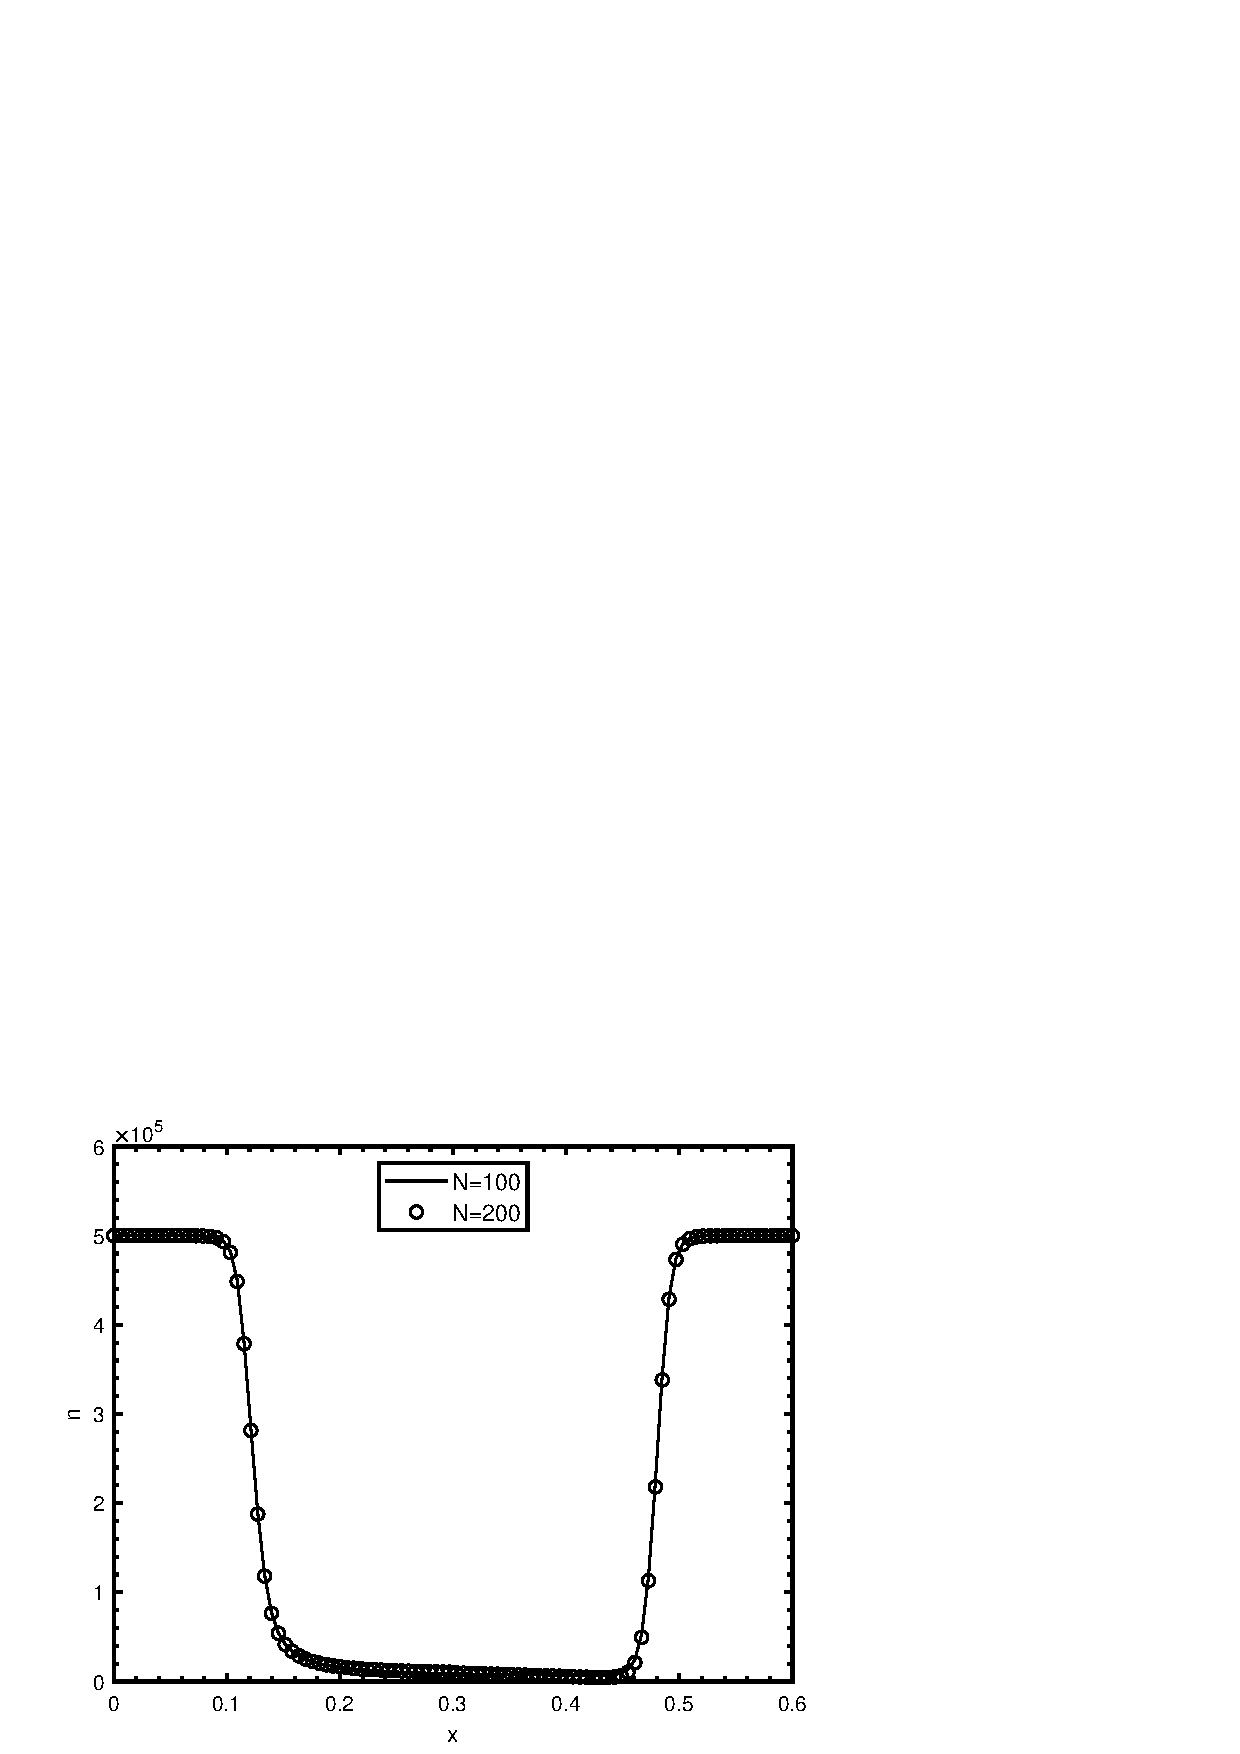
\includegraphics[width=\linewidth]{figure/DDTVDRK3Degree2mu0.75Nn.pdf}
		\end{minipage}
		\hspace{1cm}
		\begin{minipage}{0.3\linewidth}
			\centering
			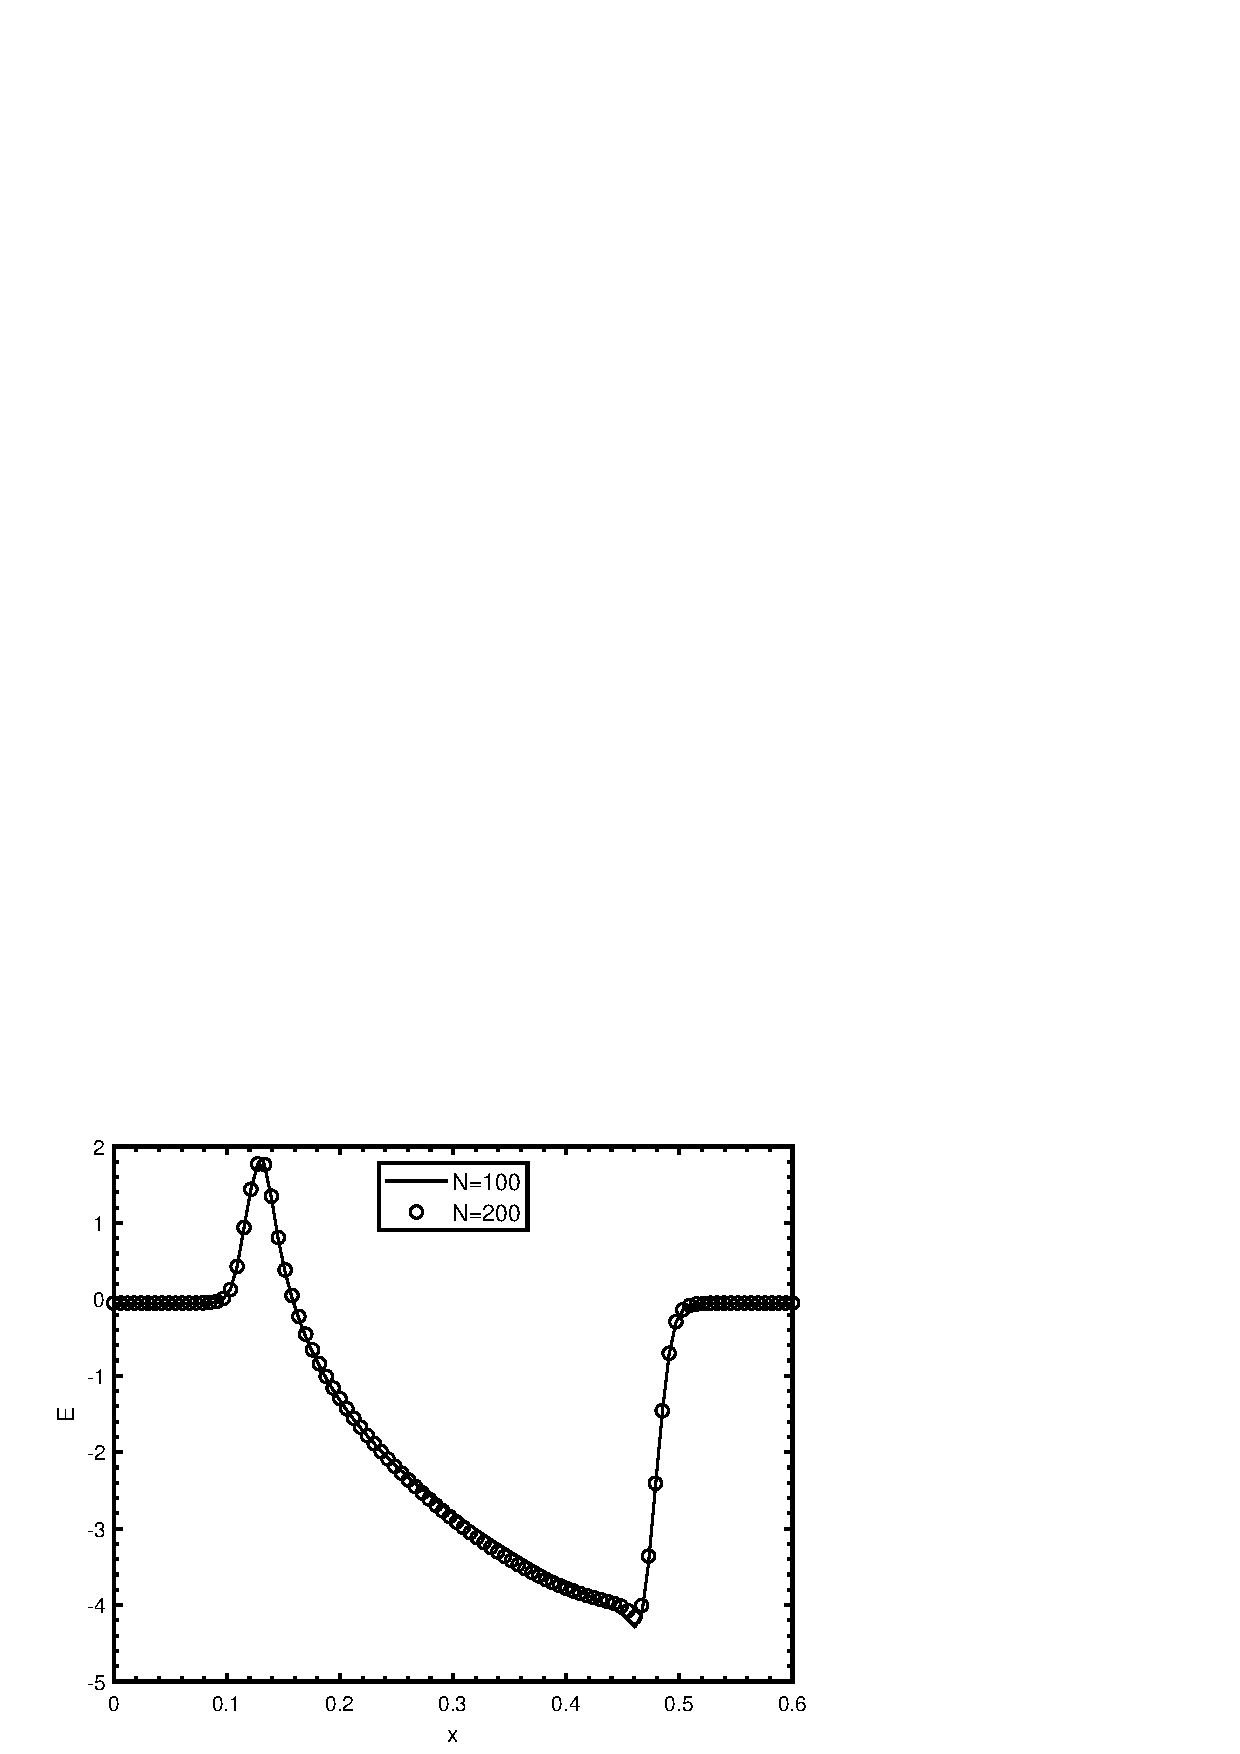
\includegraphics[width=\linewidth]{figure/DDTVDRK3Degree2mu0.75NE.pdf}
		\end{minipage}

		\centering
		\begin{minipage}{0.3\linewidth}
			\centering
			\includegraphics[width=\linewidth]{figure/DDTVDRK3Degree2N100mun.pdf}
		\end{minipage}
		\hspace{1cm}
		\begin{minipage}{0.3\linewidth}
			\centering
			\includegraphics[width=\linewidth]{figure/DDTVDRK3Degree2N100muE.pdf}
		\end{minipage}
		\caption{DD模型三阶TVDRK,计算空间$V^2$,网格数$N=100$,迁移率$\mu=0.75$。左:电子浓度n;右:电势E。}
		\label{fig:TVDRK}
	\end{figure}
\end{frame}
\begin{frame}
	上面两图基于DD模型;下面两图表示DD模型和HF模型的结果对比。
	\begin{figure}
		\centering
		\begin{minipage}{0.3\linewidth}
			\centering
			\includegraphics[width=\linewidth]{figure/DDTVDRK3Degree2N100mu0.75limitern.pdf}
		\end{minipage}
		\hspace{1cm}
		\begin{minipage}{0.3\linewidth}
			\centering
			\includegraphics[width=\linewidth]{figure/DDTVDRK3Degree2N100mu0.75limiterE.pdf}
		\end{minipage}

		\centering
		\begin{minipage}{0.3\linewidth}
			\centering
			\includegraphics[width=\linewidth]{figure/DDTVDRK3Degree2N100mu0.75modeln.pdf}
		\end{minipage}
		\hspace{1cm}
		\begin{minipage}{0.3\linewidth}
			\centering
			\includegraphics[width=\linewidth]{figure/DDTVDRK3Degree2N100mu0.75modelE.pdf}
		\end{minipage}
		\caption{三阶TVDRK,计算空间$V^2$,网格数$N=100$,迁移率$\mu=0.75$。左:电子浓度n;右:电势E。}
		\label{fig:TVDRKLimiter}
	\end{figure}
\end{frame}

\subsection{IMEX LDG格式}
\begin{frame}
	\frametitle{收敛结果}
	\begin{figure}
		\centering
		\begin{minipage}{0.3\linewidth}
			\centering
			\includegraphics[width=\linewidth]{figure/IMEXNn.pdf}
		\end{minipage}
		\hspace{1cm}
		\begin{minipage}{0.3\linewidth}
			\centering
			\includegraphics[width=\linewidth]{figure/IMEXNE.pdf}
		\end{minipage}
		\caption{默认值:DD模型三阶IMEXRK,计算空间$V^2$,网格数$N=100$和$N=200$,迁移率$\mu=0.75$。左:电子浓度n;右:电势E。}
		\label{fig:IMEX:N}
	\end{figure}
\end{frame}
\begin{frame}
	\frametitle{IMEX LDG格式的误差估计}
	\begin{equation}
		||n-n_h||_{L^{\infty}(0,T;L^2)} \leq C_1h^{k+1} + C_2 (\Delta t)^{tk} \leq C(h^{k+1} + (\Delta t)^{tk}), \quad tk = 2,3.
	\end{equation}
	\begin{table}
		\begin{tabularx}{\textwidth}{@{} *5{X} @{}}
			\toprule
			    & \multicolumn{2}{c}{$\text{IMEX2}$} & \multicolumn{2}{c}{$\text{IMEX3}$}                                                   \\
			\cmidrule(lr){2-3} \cmidrule(lr){4-5}
			N   & $\frac{||n_h-n||}{||n||}$          & Order                              & $\frac{||n_h-n||}{||n||}$ & Order               \\
			\midrule
			25  & 4.42e-03                           & \rule{\llen}{0.4pt}                & 4.42e-03                  & \rule{\llen}{0.4pt} \\
			50  & 1.21e-03                           & 1.87                               & 1.21e-03                  & 1.87                \\
			100 & 1.65e-04                           & 2.88                               & 1.65e-04                  & 2.88                \\
			200 & 2.16e-05                           & 2.93                               & 2.16e-05                  & 2.93                \\
			400 & 2.79e-06                           & 2.95                               & 2.79e-06                  & 2.95                \\
			800 & 3.41e-07                           & 3.03                               & 3.41e-07                  & 3.03                \\
			\bottomrule
		\end{tabularx}
		\caption{IMEX LDG格式误差估计。网格数N,收敛阶Order,计算空间$V^2$,时间步长$\Delta t = 1.2e-03$,相对误差$(||n_h-n||)/||n||$。}
		\label{tab:IMEXLDGerror}
	\end{table}
\end{frame}
\begin{frame}
	\frametitle{一阶IMEX LDG格式的误差估计}
	\begin{equation}
		||n-n_h||_{L^{\infty}(0,T;L^2)} + ||q - q_h||_{L^2(0,T;L^2)} \leq C(h^{k+1} + \Delta t)
	\end{equation}
	\begin{table}
		\begin{tabularx}{\textwidth}{@{} *7{X} @{}}
			\toprule
			    & \multicolumn{2}{c}{$V^0$} & \multicolumn{2}{c}{$V^1$} & \multicolumn{2}{c}{$V^2$}                                                                     \\
			\cmidrule(lr){2-3} \cmidrule(lr){4-5} \cmidrule(lr){6-7}
			N   & $||n_h-n||+||q_h-q||$     & Order                     & $||n_h-n||+||q_h-q||$     & Order               & $||n_h-n||+||q_h-q||$ & Order               \\
			\midrule
			25  & 3.04e+07                  & \rule{\slen}{0.4pt}       & 8.93e+06                  & \rule{\slen}{0.4pt} & 4.02e+06              & \rule{\slen}{0.4pt} \\
			50  & 1.96e+07                  & 0.63                      & 4.14e+06                  & 1.11                & 7.20e+05              & 2.48                \\
			100 & 1.12e+07                  & 0.81                      & 1.19e+06                  & 1.80                & 3.07e+05              & 1.23                \\
			200 & 5.87e+06                  & 0.93                      & 4.05e+05                  & 1.55                & 2.92e+05              & 0.07                \\
			400 & 2.98e+06                  & 0.98                      & 3.02e+05                  & 0.42                & 2.91e+05              & 0.00                \\
			800 & 1.52e+06                  & 0.97                      & 2.92e+05                  & 0.05                & 2.91e+05              & 0.00                \\
			\bottomrule
		\end{tabularx}
		\caption{一阶IMEX LDG格式误差估计。网格数N,收敛阶Order,计算空间$V^k, k=0,1,2$,时间步长$\Delta t = 1.2e-03$,绝对误差$||n_h-n||+||q_h-q||$。}
		\label{tab:IMEXLDGerror:1}
	\end{table}
\end{frame}
\begin{frame}
	\frametitle{二阶IMEX LDG格式的误差估计}
	\begin{equation}
		||n-n_h||_{L^{\infty}(0,T;L^2)} \leq C(h^{k+1} + (\Delta t)^2)
	\end{equation}
	\begin{table}
		\begin{tabularx}{\textwidth}{@{} *7{X} @{}}
			\toprule
			    & \multicolumn{2}{c}{$V^0$} & \multicolumn{2}{c}{$V^1$} & \multicolumn{2}{c}{$V^2$}                                                                         \\
			\cmidrule(lr){2-3} \cmidrule(lr){4-5} \cmidrule(lr){6-7}
			N   & $\frac{||n_h-n||}{||n||}$ & Order                     & $\frac{||n_h-n||}{||n||}$ & Order               & $\frac{||n_h-n||}{||n||}$ & Order               \\
			\midrule
			25  & 9.94e-02                  & \rule{\slen}{0.4pt}       & 3.23e-02                  & \rule{\slen}{0.4pt} & 4.42e-03                  & \rule{\slen}{0.4pt} \\
			50  & 5.51e-02                  & 0.85                      & 9.31e-03                  & 1.80                & 1.21e-03                  & 1.87                \\
			100 & 2.80e-02                  & 0.98                      & 2.45e-03                  & 1.92                & 1.65e-04                  & 2.88                \\
			200 & 1.41e-02                  & 0.99                      & 6.22e-04                  & 1.98                & 2.16e-05                  & 2.93                \\
			400 & 7.07e-03                  & 1.00                      & 1.58e-04                  & 1.98                & 2.79e-06                  & 2.95                \\
			800 & 3.54e-03                  & 1.00                      & 3.90e-05                  & 2.02                & 3.41e-07                  & 3.03                \\
			\bottomrule
		\end{tabularx}
		\caption{二阶IMEX LDG格式误差估计。网格数N,收敛阶Order,计算空间$V^k, k=0,1,2$,时间步长$\Delta t = 1.2e-03$,相对误差$(||n_h-n||)/||n||$。}
		\label{tab:IMEXLDGerror:2}
	\end{table}
\end{frame}
\begin{frame}
	\frametitle{三阶IMEX LDG格式的误差估计}
	\begin{equation}
		||n-n_h||_{L^{\infty}(0,T;L^2)} \leq C(h^{k+1} + (\Delta t)^3)
	\end{equation}
	\begin{table}
		\begin{tabularx}{\textwidth}{@{} *7{X} @{}}
			\toprule
			    & \multicolumn{2}{c}{$V^0$} & \multicolumn{2}{c}{$V^1$} & \multicolumn{2}{c}{$V^2$}                                                                         \\
			\cmidrule(lr){2-3} \cmidrule(lr){4-5} \cmidrule(lr){6-7}
			N   & $\frac{||n_h-n||}{||n||}$ & Order                     & $\frac{||n_h-n||}{||n||}$ & Order               & $\frac{||n_h-n||}{||n||}$ & Order               \\
			\midrule
			25  & 9.96e-02                  & \rule{\slen}{0.4pt}       & 3.23e-02                  & \rule{\slen}{0.4pt} & 4.42e-03                  & \rule{\slen}{0.4pt} \\
			50  & 5.51e-02                  & 0.85                      & 9.31e-03                  & 1.80                & 1.21e-03                  & 1.87                \\
			100 & 2.80e-02                  & 0.98                      & 2.45e-03                  & 1.92                & 1.65e-04                  & 2.88                \\
			200 & 1.41e-02                  & 0.99                      & 6.22e-04                  & 1.98                & 2.16e-05                  & 2.93                \\
			400 & 7.07e-03                  & 1.00                      & 1.58e-04                  & 1.98                & 2.79e-06                  & 2.95                \\
			800 & 3.54e-03                  & 1.00                      & 3.90e-05                  & 2.02                & 3.41e-07                  & 3.03                \\
			\bottomrule
		\end{tabularx}
		\caption{三阶IMEX LDG格式误差估计。网格数N,收敛阶Order,计算空间$V^k, k=0,1,2$,时间步长$\Delta t = 1.2e-03$,相对误差$(||n_h-n||)/||n||$。}
		\label{tab:IMEXLDGerror:3}
	\end{table}
\end{frame}

\begin{frame}
	\frametitle{计算性能}
	\begin{table}
		\centering
		\begin{tabularx}{\textwidth}{@{} *7{X} @{}}
			\toprule
			           & \multicolumn{1}{c}{TVDRK3} & \multicolumn{5}{c}{IMEX3}                                         \\
			\cmidrule(lr){2-2} \cmidrule(lr){3-7}
			\midrule
			$\Delta t$ & 1.6e-05                    & 4.0e-04                   & 6.0e-04 & 8.0e-04 & 1.0e-03 & 1.2e-03 \\
			nt         & 11457                      & 414                       & 354     & 307     & 255     & 217     \\
			t          & 0.1833                     & 0.1656                    & 0.2124  & 0.2456  & 0.2550  & 0.2604  \\
			\bottomrule
		\end{tabularx}
		\caption{TVDRK LDG格式和IMEX LDG格式达到稳态的时间步长$\Delta t$,时间层数$nt$,时间$t$。网格数$N=100$,计算空间$V^2$。}
		\label{tab:time:100}
	\end{table}
	\begin{table}
		\begin{tabularx}{\textwidth}{@{} *7{X} @{}}
			\toprule
			           & \multicolumn{1}{c}{TVDRK3} & \multicolumn{5}{c}{IMEX3}                                         \\
			\cmidrule(lr){2-2} \cmidrule(lr){3-7}
			\midrule
			$\Delta t$ & 4.2e-06                    & 4.0e-04                   & 6.0e-04 & 8.0e-04 & 1.0e-03 & 1.2e-03 \\
			nt         & 39892                      & 416                       & 353     & 307     & 255     & 217     \\
			t          & 0.1675                     & 0.1664                    & 0.2118  & 0.2456  & 0.2550  & 0.2604  \\
			\bottomrule
		\end{tabularx}
		\caption{TVDRK LDG格式和IMEX LDG格式达到稳态的时间步长$\Delta t$,时间层数$nt$,时间$t$。网格数$N=200$,计算空间$V^2$。}
		\label{tab:time:200}
	\end{table}
\end{frame}


%%%%%%%%%%%%%
% 总结与展望
%%%%%%%%%%%%%
\section{总结与展望}
\begin{frame}
	\frametitle{总结与展望}
	\begin{itemize}
		\item 根据数值算例的结果,我们证明了TVD LDG格式和IMEX LDG格式收敛性,以及IMEX LDG格式的无条件稳定性。并证明了IMEX LDG格式误差分析的正确性。
		\item 由于结果中时间项的影响远小于空间项,未来可以考虑求出时间项和空间项系数的显式表达式,来获得更加精确的误差估计。在此基础上我们可以更精确地选择时间步长。
		\item 这些数值方法也有望应用于其他物理模型。
	\end{itemize}
\end{frame}
%%%%%%%%%%%%%
% 参考文献
%%%%%%%%%%%%%
\begin{frame}{参考文献}
	\printbibliography
\end{frame}

%%%%%%%%%%%%%
% 鸣谢
%%%%%%%%%%%%%

\begin{frame}
	\frametitle{鸣谢}
	\Huge
	\begin{center}
		谢谢!
	\end{center}
\end{frame}
\end{document}